\documentclass[border={0.1cm 0.1cm 0.1cm 0.1cm}]{standalone}  %E,S,W,N

\usepackage{amssymb}
\usepackage{amsmath}
%\usepackage{graphicx}
\usepackage{tikz}
\usetikzlibrary{shapes} %for node shapes
\usetikzlibrary{calc}	%for centerarc
\usetikzlibrary{arrows, arrows.meta} %for big arrowhead
\usepackage{cancel}		%for strikethrough $

\def\centerarc[#1](#2)(#3:#4:#5) {\draw[#1] ($(#2)+({#5*cos(#3)},{#5*sin(#3)})$) arc (#3:#4:#5);}

%by Jean-Jacques Pinto (1978)
%https://hal.archives-ouvertes.fr/hal-01451328/file/Schema-R-revu-par-Jean-Jacques-Pinto.pdf

\begin{document}
	
	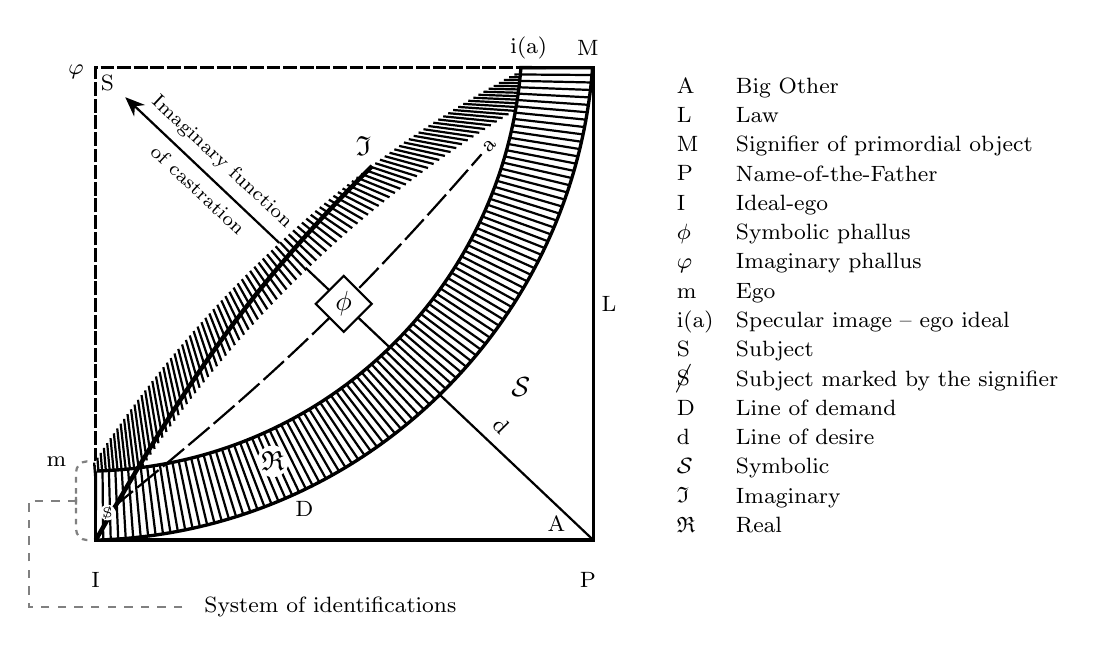
\begin{tikzpicture}[thick]
	%SQUARE
	\draw[very thick,dash pattern=on 5 off 1] (0,1)--(0,6)--(5.5,6);
	\draw[very thick] (0,0.95)--(0,0)--(6.32,0)--(6.32,6)--(5.5,6);
	\draw[-{Stealth[length=2.5mm,width=2mm]}] (6.32,0)--(0.375,6-0.375);
	
	%SMALL ARC
	%\draw (0,0) arc (151:117:14.75cm);
	%\draw (0,0) arc (-88.5:-5:6.5cm);
	\fill[white] (0,1) arc (147:117.9:14.75cm)--(6.28,6) arc (116.5:150.6:14.75cm)--cycle;
	\centerarc[very thick](12.35,-7.05)(147:117.9:14.75cm)
	\centerarc[very thick](12.9,-7.2)(116.5:150.6:14.75cm)
	\foreach \i in {0,...,100} \draw ({12.35+14.75*cos(147-0.291*\i)},{-7.05+14.75*sin(147-0.291*\i)})-- ({12.9+14.75*cos(150.6-0.341*\i)},{-7.2+14.75*sin(150.6-0.341*\i)}); %hatching
	
	%BIG ARC
	\fill[white,draw=black,very thick] (0,0) arc (-88.5:-4.4:6.5cm)--(5.4,6) arc (-4.4:-88.5:5.55cm);
	\foreach \i in {0,...,100} \draw ({-0.14+5.55*cos(-88.5+0.841*\i)},{6.42+5.55*sin(-88.5+0.841*\i)})-- ({-0.17+6.5*cos(-88.5+0.841*\i)},{6.5+6.5*sin(-88.5+0.841*\i)}); %hatching
	%\centerarc[green](-0.14,6.42)(-4.4:-88.5:5.55cm)
	%\centerarc[blue](-0.17,6.5)(-88.5:-4.4:6.5cm)
	\draw[ultra thick] (0,0) to[out=60,in=225] (3.51,4.75); %weird line that overlaps both arcs
	\fill[white] (2.25,1) circle (0.2cm) node[black] {$\mathfrak{\small R}$};
	%
	\draw[dash pattern=on 10 off 2] (0.2,0.4) to[out=39,in=229] (5-0.1,5-0.1); %diagonal dash line
	\node[diamond,fill=white,draw=black,inner sep=0.5mm] at (3.15,3) {$\phi$};
	%
	\fill[white] (0.15,0.35) circle (0.1cm) node[black] {\tiny S};
	\draw[very thin] (0.15-0.03,0.35-0.08)--(0.15+0.03,0.35+0.08); %kludge strikethrough
	
	%LABELS
	\node at (2.65,0.4) {\footnotesize D};
	\node at (5.4,1.95) {$\mathcal{\small S}$};
	\node at (5.15,1.45) {\rotatebox{-45}{\footnotesize d}};
	\node at (5,5) {\rotatebox{45}{\footnotesize a}};
	\node at (5.85,0.2) {\footnotesize A};
	\node at (0.15,5.8) {\footnotesize S};
	\node at (-0.25,5.95) {\footnotesize $\varphi$};
	\node at (3.4,5) {$\mathfrak{\small I}$};
	\node at (1.6,4.8) {\rotatebox{-43}{\scriptsize Imaginary function}};
	\node at (1.3,4.45) {\rotatebox{-43}{\scriptsize of castration}};
	\node at (0,-0.5) {\footnotesize I};
	\node at (6.25,-0.5) {\footnotesize P};
	\node at (6.52,3) {\footnotesize L};
	\node at (6.25,6.25) {\footnotesize M};
	\node at (5.5,6.25) {\footnotesize i(a)};
	\node at (-0.5,1) {\footnotesize m};
	\node[right] at (1.25,-0.85) {\footnotesize System of identifications};
	\draw[dashed,gray] (1.1,-0.85)--(-0.85,-0.85)--(-0.85,0.5)--(-0.15,0.5);
	%\draw[dashed] (-0.25,0.5) to[bend left] (0,1);
	%\draw[dashed] (-0.25,0.5) to[bend right] (0,0);
	\draw[dashed,rounded corners,dash pattern=on 2 off 2,gray] (-0.25,0.5-0.05)--(-0.25,1)--(-0.05,1);
	\draw[dashed,rounded corners,dash pattern=on 2 off 2,gray] (-0.25,0.5+0.05)--(-0.25,0)--(-0.05,0);
	
	%LEGEND
	\node[align=left,below right] at (7.25,6) {\footnotesize%
		A\\[-0.5mm]\footnotesize
		L\\[-0.5mm]\footnotesize
		M\\[-0.5mm]\footnotesize
		P\\[-0.5mm]\footnotesize
		I\\[-0.5mm]\footnotesize
		$\phi$\\[-0.5mm]\footnotesize
		$\varphi$\\[-0.5mm]\footnotesize
		m\\[-0.5mm]\footnotesize
		i(a)\\[-0.5mm]\footnotesize
		S\\[-0.5mm]\footnotesize
		\cancel{S}\\[-0.5mm]\footnotesize
		D\\[-0.5mm]\footnotesize
		d\\[-0.5mm]\footnotesize
		$\mathcal{S}$\\[-0.5mm]\footnotesize
		$\mathfrak{I}$\\[-0.5mm]\footnotesize
		$\mathfrak{R}$
	};
	
	\node[align=left,below right] at (8,6) {\footnotesize%
		Big Other \\[-0.5mm]\footnotesize
		Law \\[-0.5mm]\footnotesize
		Signifier of primordial object \\[-0.5mm]\footnotesize
		Name-of-the-Father \\[-0.5mm]\footnotesize
		Ideal-ego \\[-0.5mm]\footnotesize
		Symbolic phallus \\[-0.5mm]\footnotesize
		Imaginary phallus \\[-0.5mm]\footnotesize
		Ego \\[-0.5mm]\footnotesize
		Specular image -- ego ideal \\[-0.5mm]\footnotesize
		Subject \\[-0.5mm]\footnotesize
		Subject marked by the signifier \\[-0.5mm]\footnotesize
		Line of demand \\[-0.5mm]\footnotesize
		Line of desire \\[-0.5mm]\footnotesize
		Symbolic \\[-0.5mm]\footnotesize
		Imaginary \\[-0.5mm]\footnotesize
		Real
	};
	\end{tikzpicture}
	
\end{document}